\documentclass[16pts]{report}
\usepackage[utf8]{inputenc}
\usepackage[T1]{fontenc}
\usepackage[francais]{babel}
\usepackage{xcolor}
\usepackage[hyphens]{url}
\usepackage[hidelinks]{hyperref}
\usepackage{amsmath}
\usepackage{graphicx}
\usepackage{geometry}
\usepackage{textcomp}
\usepackage{tabularx}
\hypersetup{hypertexnames=true}
\geometry{hmargin=2.5cm,vmargin=1.5cm}

\usepackage{float} %Option H pour les figures, utile.

%\maketitle
%\clearpage

\begin{document}
\bibliographystyle{unsrt}
\nocite{*}

\chapter{Architecture}
\label{cha:Architecture}

Nous avons choisi de regrouper chacun de nos modules dans différents fichiers.
Chaque fichier contient les fonctions et les attributs de ses modules. Le nom
des fonctions comporte le nom du module auquel elles sont rattachées en
préfixe.

On peut constater que certains de ces fichiers ne comportent qu’une fonction.
Cependant, il existe des fonctions privées qui ne sont pas représentées dans le
diagramme (c.f. plus bas) et cette conception nous semble être la plus adéquate
puisqu’elle nous permettra d’ajouter de nouvelles fonctions simplement, si cela
s'avère nécessaire, et ce avec un minimum de modification dans l’architecture.

\begin{figure}[H]
    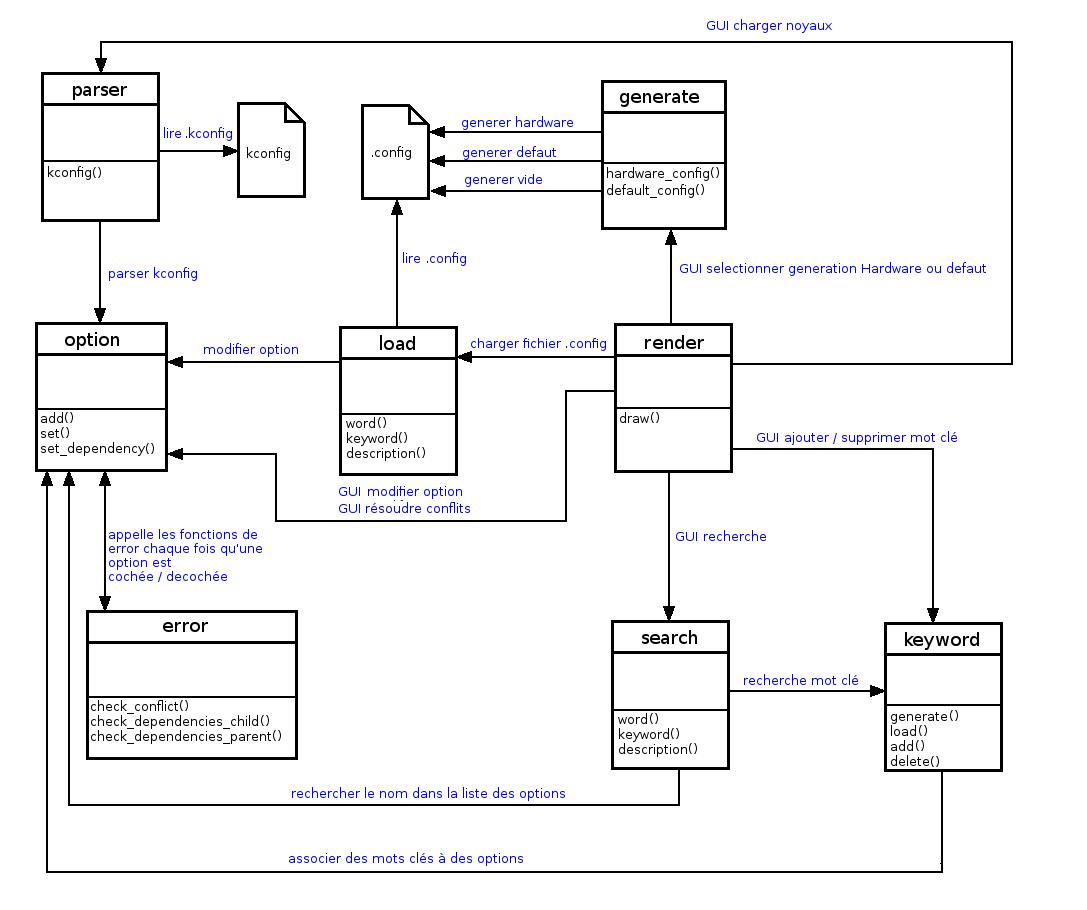
\includegraphics[scale=0.5]{illustrations/diagramme_architecture.png}
    \centering
    \caption{Diagramme des modules}
    \label{fig:DMod}
\end{figure}


Les explications sur chaque module sont données ci-après.

\chapter{Fichier keyword.h}
\label{cha:Fichier keyword.h}
Toutes les fonctions concernant les mots clés sont regroupées dans le fichier
keyword. Les fonctions de ce fichier seront appelées lorsque l’utilisateur
voudra ajouter ou enlever un mot-clé rattaché à une option. La liste des
mots-clés sera également consultée lors d’une recherche (pour trouver les
options associées à un ou plusieurs mots-clés).

\section{keyword\textunderscore generate}
\label{sec:keyword generate}
\begin{description}
    \item[input] Vide
    \item[action] Création du fichier (vierge)
    \item[output] Code d’erreur (ou de validation) $\rightarrow$ La valeur de
        retour permet de vérifier par exemple si le fichier existe déjà, si la
        création a échoué à cause des droits, à cause de l’espace disque, etc.
\end{description}

\section{keyword\textunderscore load}
\label{sec:keyword load}
\begin{description}
    \item[input] Un fichier (disque)
    \item[action] Charge le fichier en mémoire
    \item[output] Code d'erreur (ou de validation)
\end{description}

\section{keyword\textunderscore add}
\label{sec:keyword add}
\begin{description}
    \item[input] Une option, une chaîne de caractère
    \item[action] Ajoute un mot-clé à la liste des mots-clés
    \item[output] Code d'erreur (ou de validation)
\end{description}

\section{keyword\textunderscore delete}
\label{sec:keyword delete}
\begin{description}
    \item[input] Une option, une chaîne de caractère
    \item[action] Supprime un mot-clé à la liste des mots-clés
    \item[output] Code d'erreur (ou de validation)
\end{description}


\chapter{Fichier parser.h}
\label{cha:Fichier parser.h}
Le module parser regroupe toutes les fonctions et attributs servant à parser un
fichier kconfig. L’utilité de ce module et de lire un fichier kconfig et de
crée la liste des options de ce kconfig. Les fonctions de ce module seront
appelées lors du chargement du noyau (Maquette 1).

\section{parser\textunderscore kconfig}
\label{sec:parser kconfig}
\begin{description}
    \item[input] Un fichier Kconfig
    \item[action] Charge en mémoire la liste des options du kconfig, c’est à
        dire les options compatibles avec le noyau sélectionné
    \item[output]
    \begin{itemize}
        \item Code d'erreur (ou de validation)
        \item Liste de toutes les options du noyau
    \end{itemize}
\end{description}


\chapter{Fichier generate.h}
\label{cha:Fichier generate.h}
Les trois premières fonctions de ce module sont appelées lors de la sélection
du mode de configuration du noyau (Maquette 2). Elles servent à générer un
.config préliminaire que l’application pourra charger, et que l’utilisateur
pourra modifier.
La dernière fonction sauvegarde le fichier .config courant.

\section{generate\textunderscore hardware\textunderscore config}
\label{sec:generate hardware config}
\begin{description}
    \item[input] Vide
    \item[action] Scanne le matériel présent sur la machine, et génère un
        fichier .config contenant les options devant être activées pour être
        compatibles avec ce matériel.
    \item[output] Un fichier .config
\end{description}

\section{generate\textunderscore default\textunderscore config}
\label{sec:generate default config}
\begin{description}
    \item[input] Vide
    \item[action] Exécute la commande "make defconfig"
    \item[output] Liste des options par défaut
\end{description}

\section{generate\textunderscore empty\textunderscore config}
\label{sec:generate empty config}
\begin{description}
    \item[input] Vide
    \item[action] Création d'un fichier vierge
    \item[output] Un fichier .config vierge, vide de toute option
\end{description}

\section{generate\textunderscore current\textunderscore config}
\label{sec:generate current config}
\begin{description}
    \item[input] Emplacement de la sauvegarde
    \item[action] Sauvegarde du .config courant
    \item[output] Le fichier .config final
\end{description}

\chapter{Fichier load.h}
\label{cha:Fichier load.h}
La fonction load\_config de ce module sera appelée pour charger en mémoire un
fichier .config. Celui-ci contient une liste d’options ayant pour valeurs YES
(en dur) et MOD (en module) (les options non sélectionnées ne sont pas
représentées). La fonction changera les valeurs des options en mémoire pour les
faire correspondre à cette liste.

\section{load\textunderscore config}
\label{sec:load config}
\begin{description}
    \item[input] Le chemin (ou le nom) vers un fichier .config, et la liste des
        options en mémoire
    \item[action] Coche les options chargées en mémoire (voir parser\_kconfig)
        qui sont dans le fichier .config
    \item[output]
    \begin{itemize}
        \item Code d'erreur (ou de validation)
        \item Liste des options (en mémoire)
    \end{itemize}
\end{description}

\textit{Note d’implémentation} : Comment faire la correspondance entre un fichier
.config et les options en mémoire sans avoir à parcourir toutes les options
en mémoire à chaque fois ?


\chapter{Fichier render.h}
\label{cha:Fichier render.h}
Le module render gère l’interface graphique (GTK), il s’occupera de dessiner
l’interface et de récupérer les évènements du clavier et de la souris. Tous les
autres modules sont directement liés à render, car ils seront susceptibles
d’être appelés lorsqu’une action (clavier ou souris) sera détectée dans render.

\section{render\textunderscore draw}
\label{sec:render draw}
\begin{description}
    \item[input] Non défini
    \item[action] Met à jour l'affichage
    \item[output] Vide
\end{description}

\section{render\textunderscore get\textunderscore event}
\label{sec:render get event}

\begin{description}
    \item[input] Événement
    \item[action] Détermine l'événement en cours (clique sur un bouton / pression
        sur une touche / etc ...)
    \item[output] Nature de l'événement
\end{description}

\section{Fichier option.h}
\label{sec:Fichier option.h}
L'implémentation de la structure option (contenu dans ce fichier) reste encore
à débattre.

\section{option\textunderscore create}
\label{sec:option create}
\begin{description}
    \item[input]
        \begin{itemize}
            \item Nom de l'option
            \item Valeur (YES / NO / MOD)
            \item Liste des dépendances père
            \item Liste des dépendances fils
            \item Liste des options conflits
        \end{itemize}
    \item[action] Crée une structure option
    \item[output] Structure option
\end{description}

\section{option\textunderscore add}
\label{sec:option add}
\begin{description}
    \item[input] Liste des options, option à ajouter
    \item[action] Ajoute l'option à la liste d'option
    \item[output] Vide
\end{description}

\section{option\textunderscore del}
\label{sec:option del}
\begin{description}
    \item[input] Liste des options, option à retirer
    \item[action] Supprime l'option à la liste d'option
    \item[output] Vide
\end{description}

\section{option\textunderscore set (YES / NO / MOD)}
\label{sec:option set (YES / NO / MOD)}
\begin{description}
    \item[input] Liste des options, option concernée
    \item[action] Met à jour l’état d’une option en fonction du paramètre
    \item[output] Vide
\end{description}

\section{option\textunderscore set\textunderscore dependencies (YES / NO / MOD)}
\label{sec:option set dependencies (YES / NO / MOD)}
\begin{description}
    \item[input] Liste des options, option concernée
    \item[action] Met à jour l’état d’une option et de ses dépendances en fonction du paramètre
    \item[output] Vide
\end{description}


\chapter{Fichier search.h}
\label{cha:Fichier search.h}

Dans ce module sont rassemblées les fonctions qui permettront à l’utilisateur
de rechercher une option via un titre, un mot-clé ou une description. Elles
renvoient la liste des options qui correspond aux critères de recherche.

\section{search\textunderscore word}
\label{sec:search word}
\begin{description}
    \item[input] Chaîne de caractère (mot)
    \item[action] Cherche dans la liste des options, l’option représentée par son nom
    \item[output] La liste des options correspondantes aux critères de recherche
\end{description}

\section{search\textunderscore keyword}
\label{sec:search keyword}
\begin{description}
    \item[input] Chaîne de caractère (mot clé)
    \item[action] Cherche dans la liste des options, l’option est représentée par un de ses mots-clés
    \item[output] La liste des options correspondantes aux critères de recherche
\end{description}

\section{search\textunderscore description}
\label{sec:search description}
\begin{description}
    \item[input] Chaîne de caractère (mot)
    \item[action] Cherche dans la liste des options, l’option représentée par un mot dans sa description
    \item[output] La liste des options correspondantes aux critères de recherche
\end{description}


\chapter{Fichier error.h}
\label{cha:Fichier error.h}
Les fonctions du fichier error sont appelées Lesorsque l’utilisateur coche ou
décoche une option. \\
Si une option est cochée il faut :
\begin{itemize}
    \item Vérifier qu’elle ne rentre pas en conflit avec une autre option
        (error\_check\_conflict).
    \item Vérifier que ses options parents (options dont dépend celle-ci)
        soient cochées (error\_check\_dependencies\_parent).
\end{itemize}

Si une option est décochée il faut :
\begin{itemize}
    \item Vérifier que ses options enfants (options qui dépendndent de
        celle-ci) soient décochées).
\end{itemize}

Le résultat de ces fonctions est renvoyé au module option qui tentera de
résoudre automatiquement les conflits (ou problèmes de dépendances).

\section{error\textunderscore check\textunderscore conflict}
\label{sec:error check conflict}
\begin{description}
    \item[input] Option
    \item[action] Détermine s’il y a un conflit après avoir coché cette option
    \item[output] TRUE / FALSE
\end{description}

\section{error\textunderscore dependencies\textunderscore child}
\label{sec:error dependencies child}
\begin{description}
    \item[input] Option
    \item[action] Détermine si toutes les dépendances enfants sont activées.
    \item[output] TRUE / FALSE
\end{description}

\section{error\textunderscore dependencies\textunderscore parent}
\label{sec:error dependencies parent}
\begin{description}
    \item[input] Option
    \item[action] Détermine si toutes les dépendances parents sont activées.
    \item[output] TRUE / FALSE
\end{description}

\chapter{Structure de données}
\label{cha:Structure de données}


Nous allons utiliser plusieurs structures de données dans ce projet afin de
stocker différentes informations. La structure la plus importante est celle qui
correspond aux options qui nous permettra de gérer les conflits en sachant par
exemple les options qui dépendent ou qui sont dépendantes d’une option. Le
contenu de ces structures n’est pas exhaustif.

\section{option\textunderscore t}
\label{sec:option t}

\begin{tabularx}{\textwidth}{|c|X|X|c|}
\hline
nom & type & description & exemple \\
\hline
\hline
name & char* (64) & nom de l'option & CRYPTO\_AES\_586 \\
\hline
value & int & valeur de l'option (YES / NO / MOD) & YES \\
\hline
child & opiton\_t** & liste d'option dépendantes de l'option courante & \\
\hline
parent & option\_t** & liste d'option dont dépend l'option courante & \\
\hline
conflict & option\_t** & liste d'option entrant en conflit avec l'option courante &   \\
\hline
\end{tabularx}

\section{option\textunderscore keyword\textunderscore t}
\label{sec:option keyword t}

\begin{tabular}{|c|c|c|c|}
\hline
nom & type & description & exemple \\
\hline
\hline
option & option\_t & option associé au mot-clé & \\
\hline
keyword & char* (64) & mot-clé associé à l'option & CRYPTO \\
\hline
\end{tabular}


\end{document}
